%% This is an example first chapter.  You should put chapter/appendix that you
%% write into a separate file, and add a line \include{yourfilename} to
%% main.tex, where `yourfilename.tex' is the name of the chapter/appendix file.
%% You can process specific files by typing their names in at the 
%% \files=
%% prompt when you run the file main.tex through LaTeX.

\singlespacing{

\chapter{Design}

\begin{figure}
  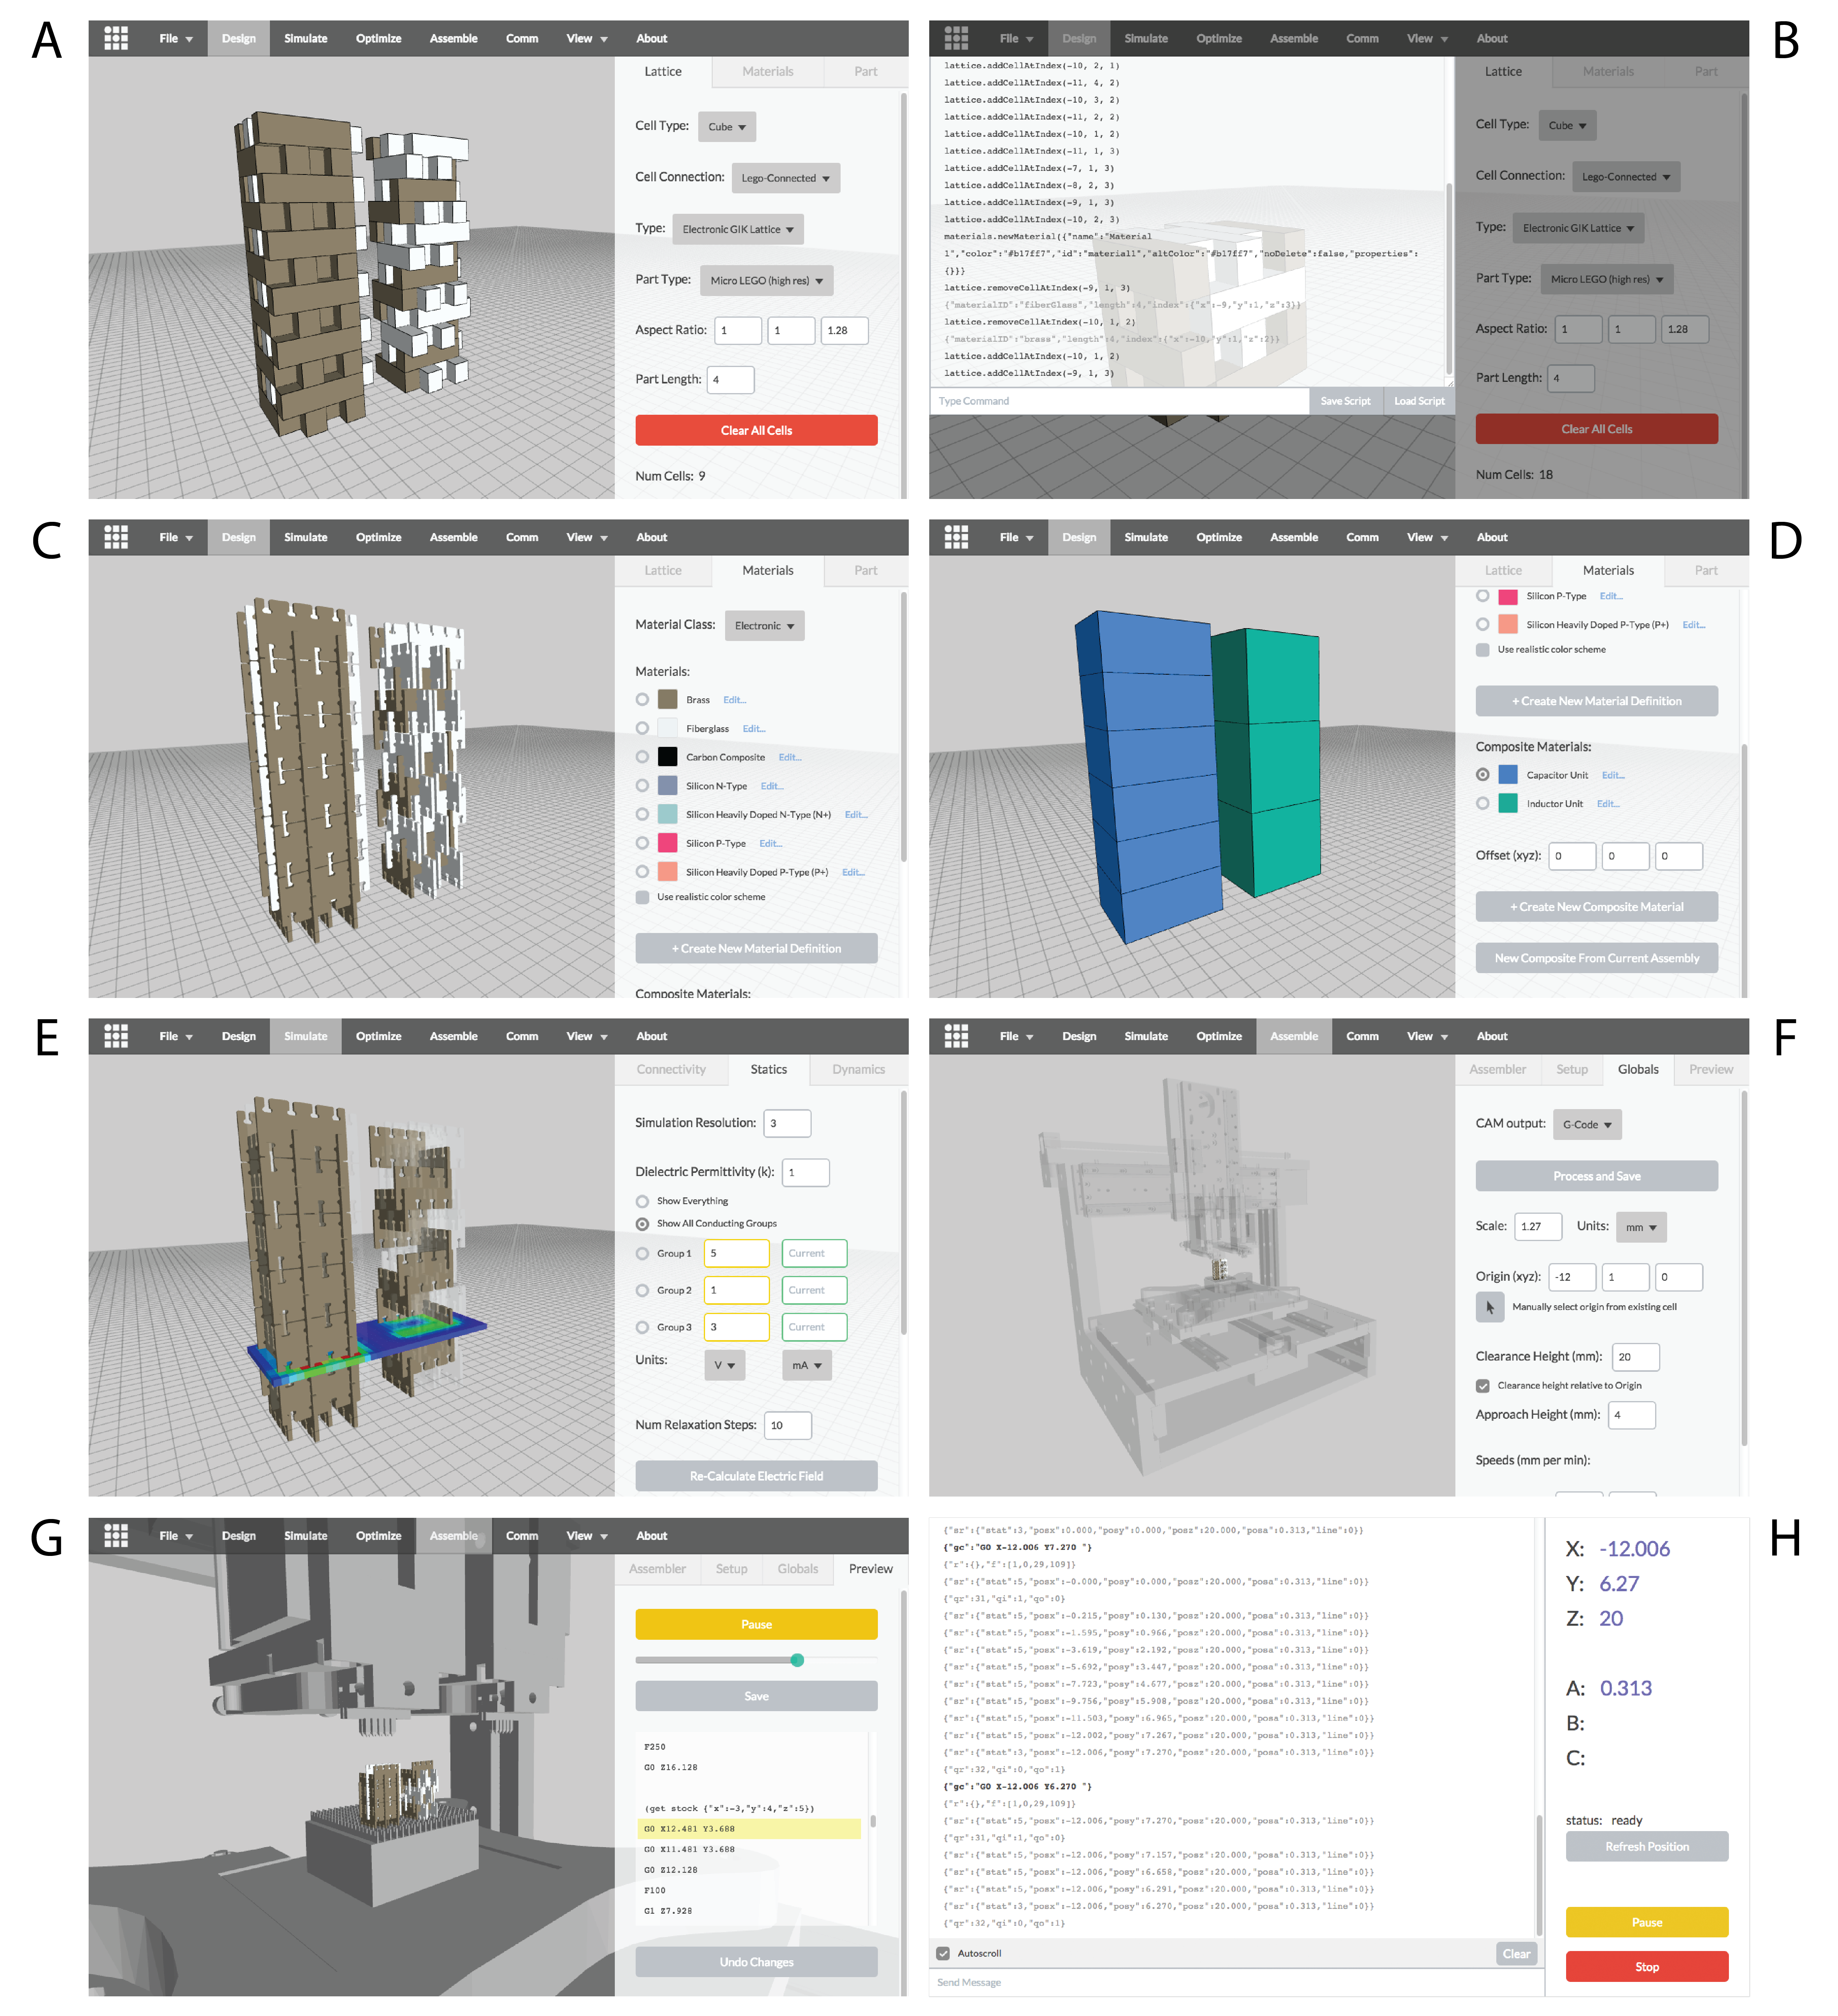
\includegraphics[width=\linewidth]{20151215DMDesignscreenshotsx8.png}
  \caption{20151215DMDesignscreenshotsx8.}
  \label{fig:DMDesignscreenshotsx8}
\end{figure}


\section{Part Abstraction}

\begin{figure}
  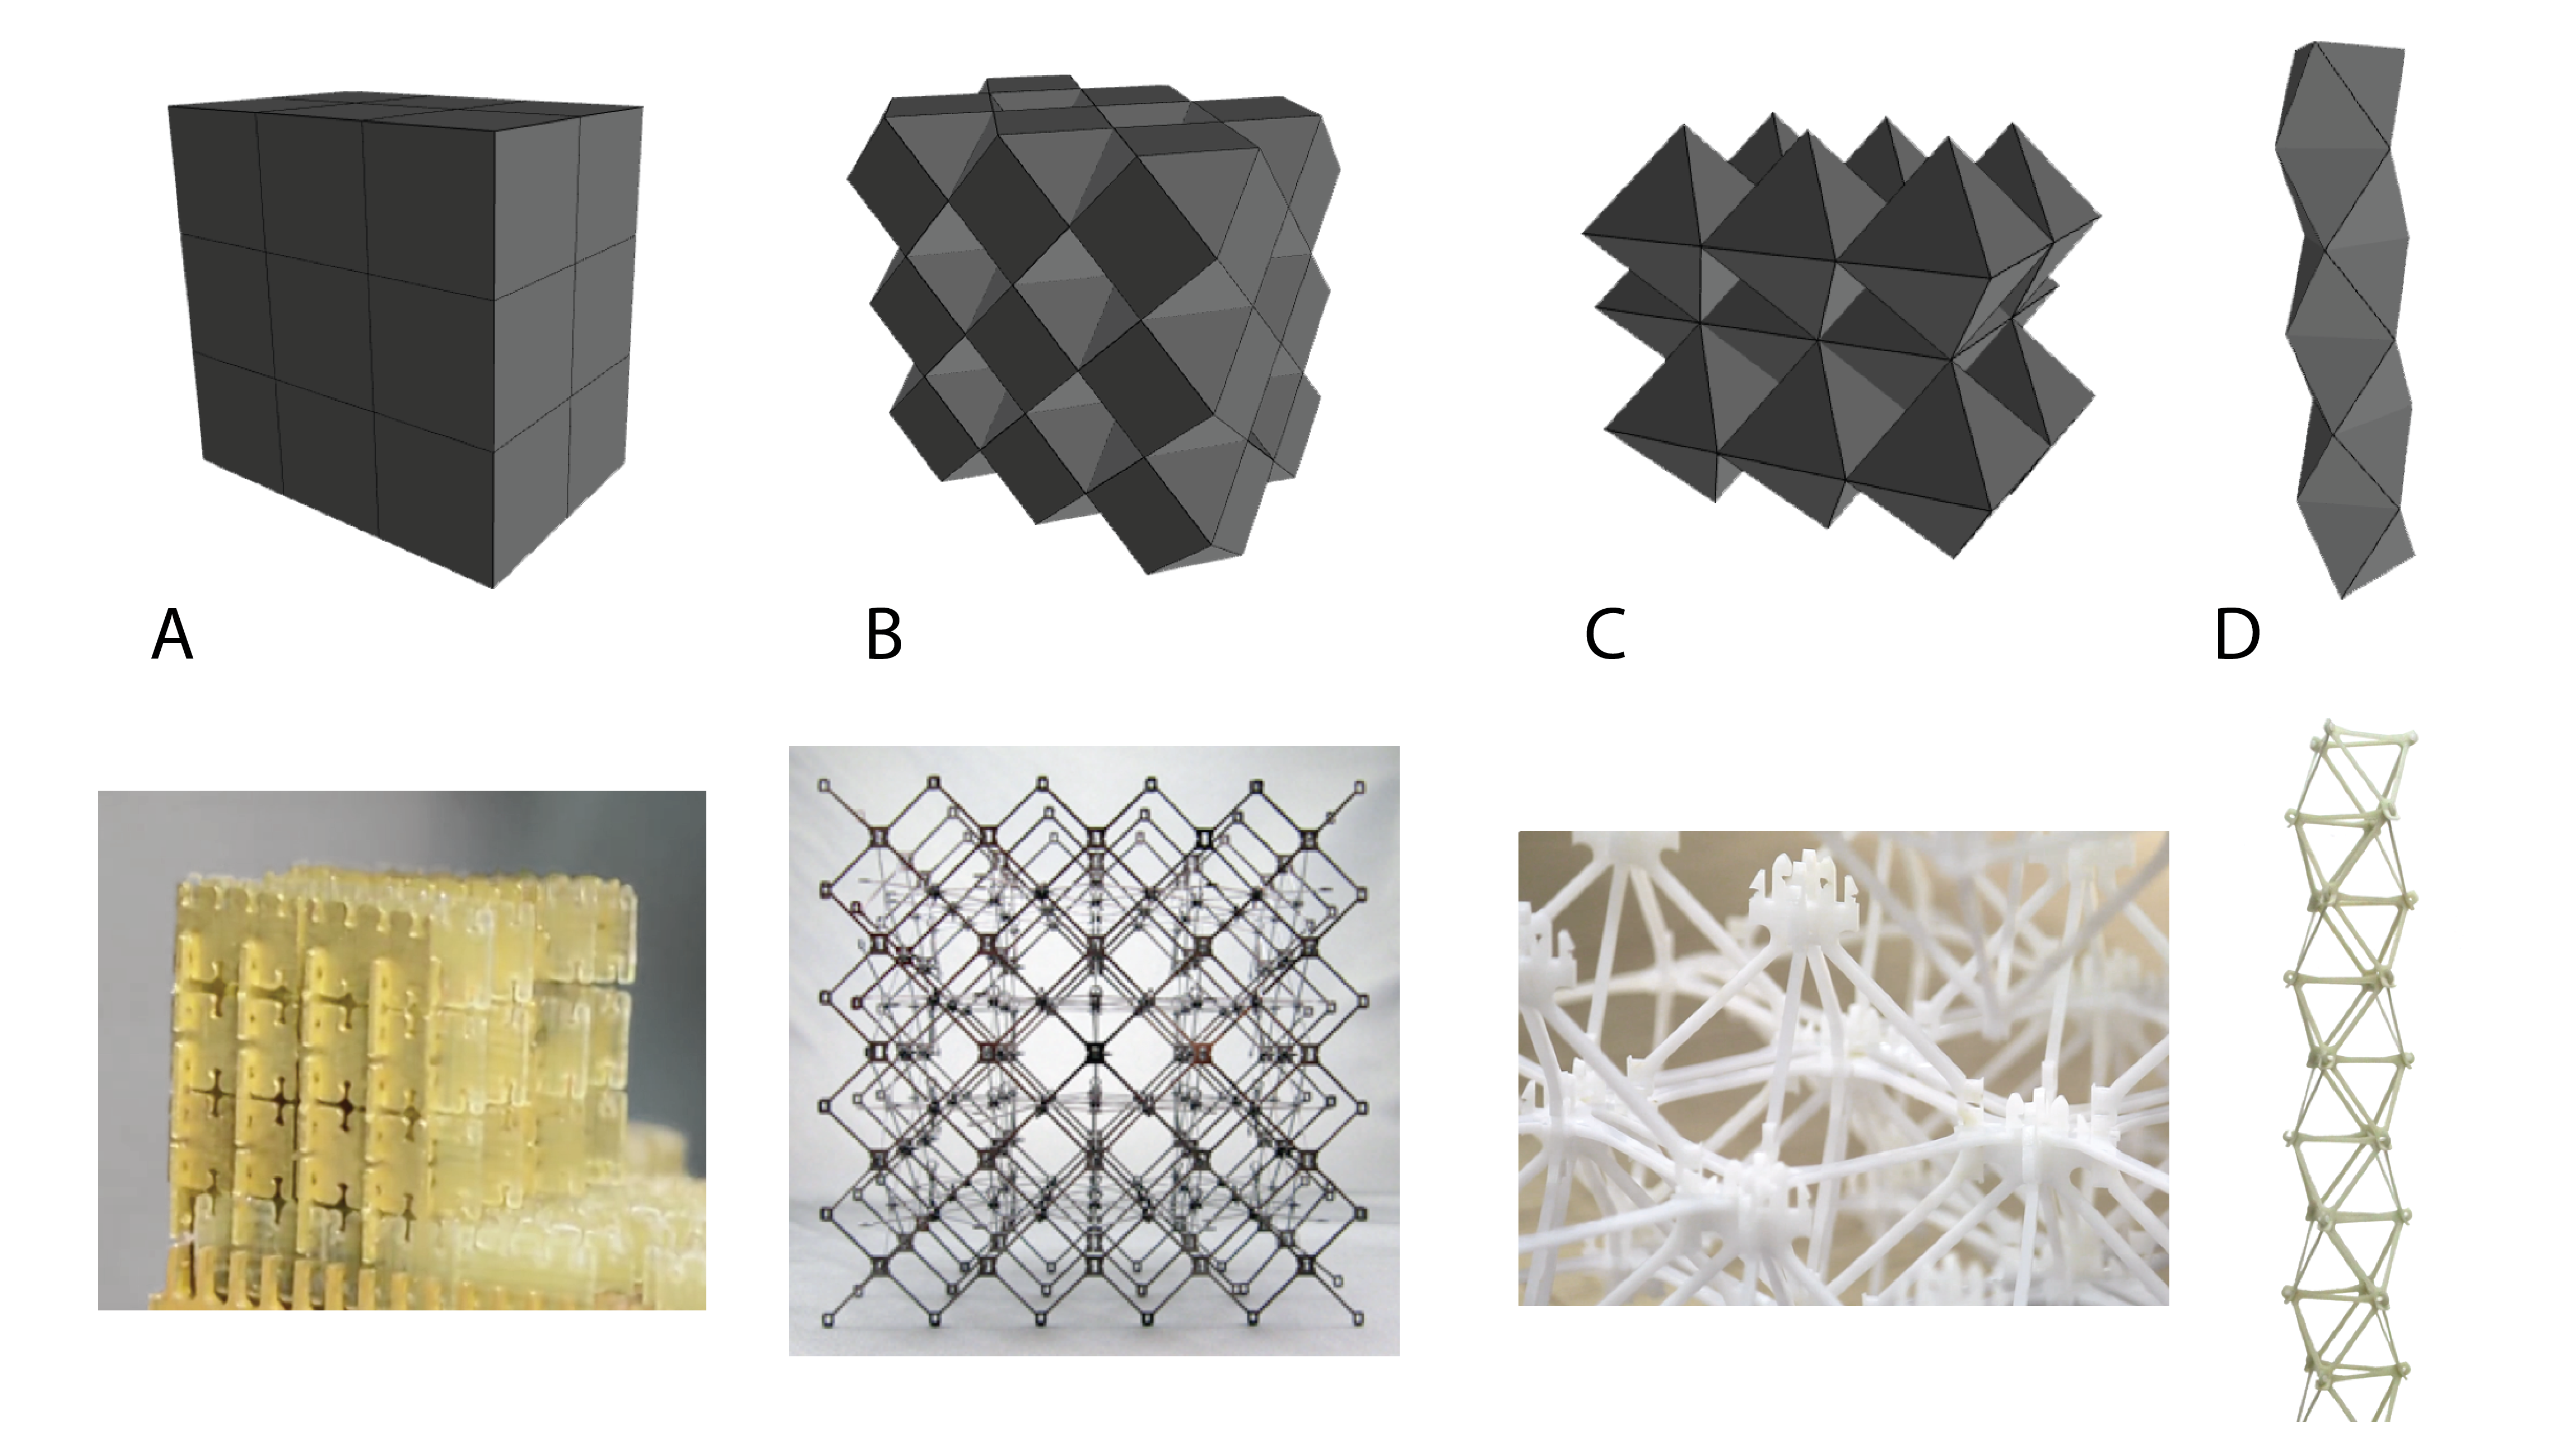
\includegraphics[width=\linewidth]{MechanicalLattices.png}
  \caption{MechanicalLattices.png.}
  \label{fig:MechanicalLattices}
\end{figure}

\begin{figure}
  \includegraphics[width=\linewidth]{PartAbstraction.png}
  \caption{PartAbstraction.png.}
  \label{fig:PartAbstraction}
\end{figure}

\begin{figure}
  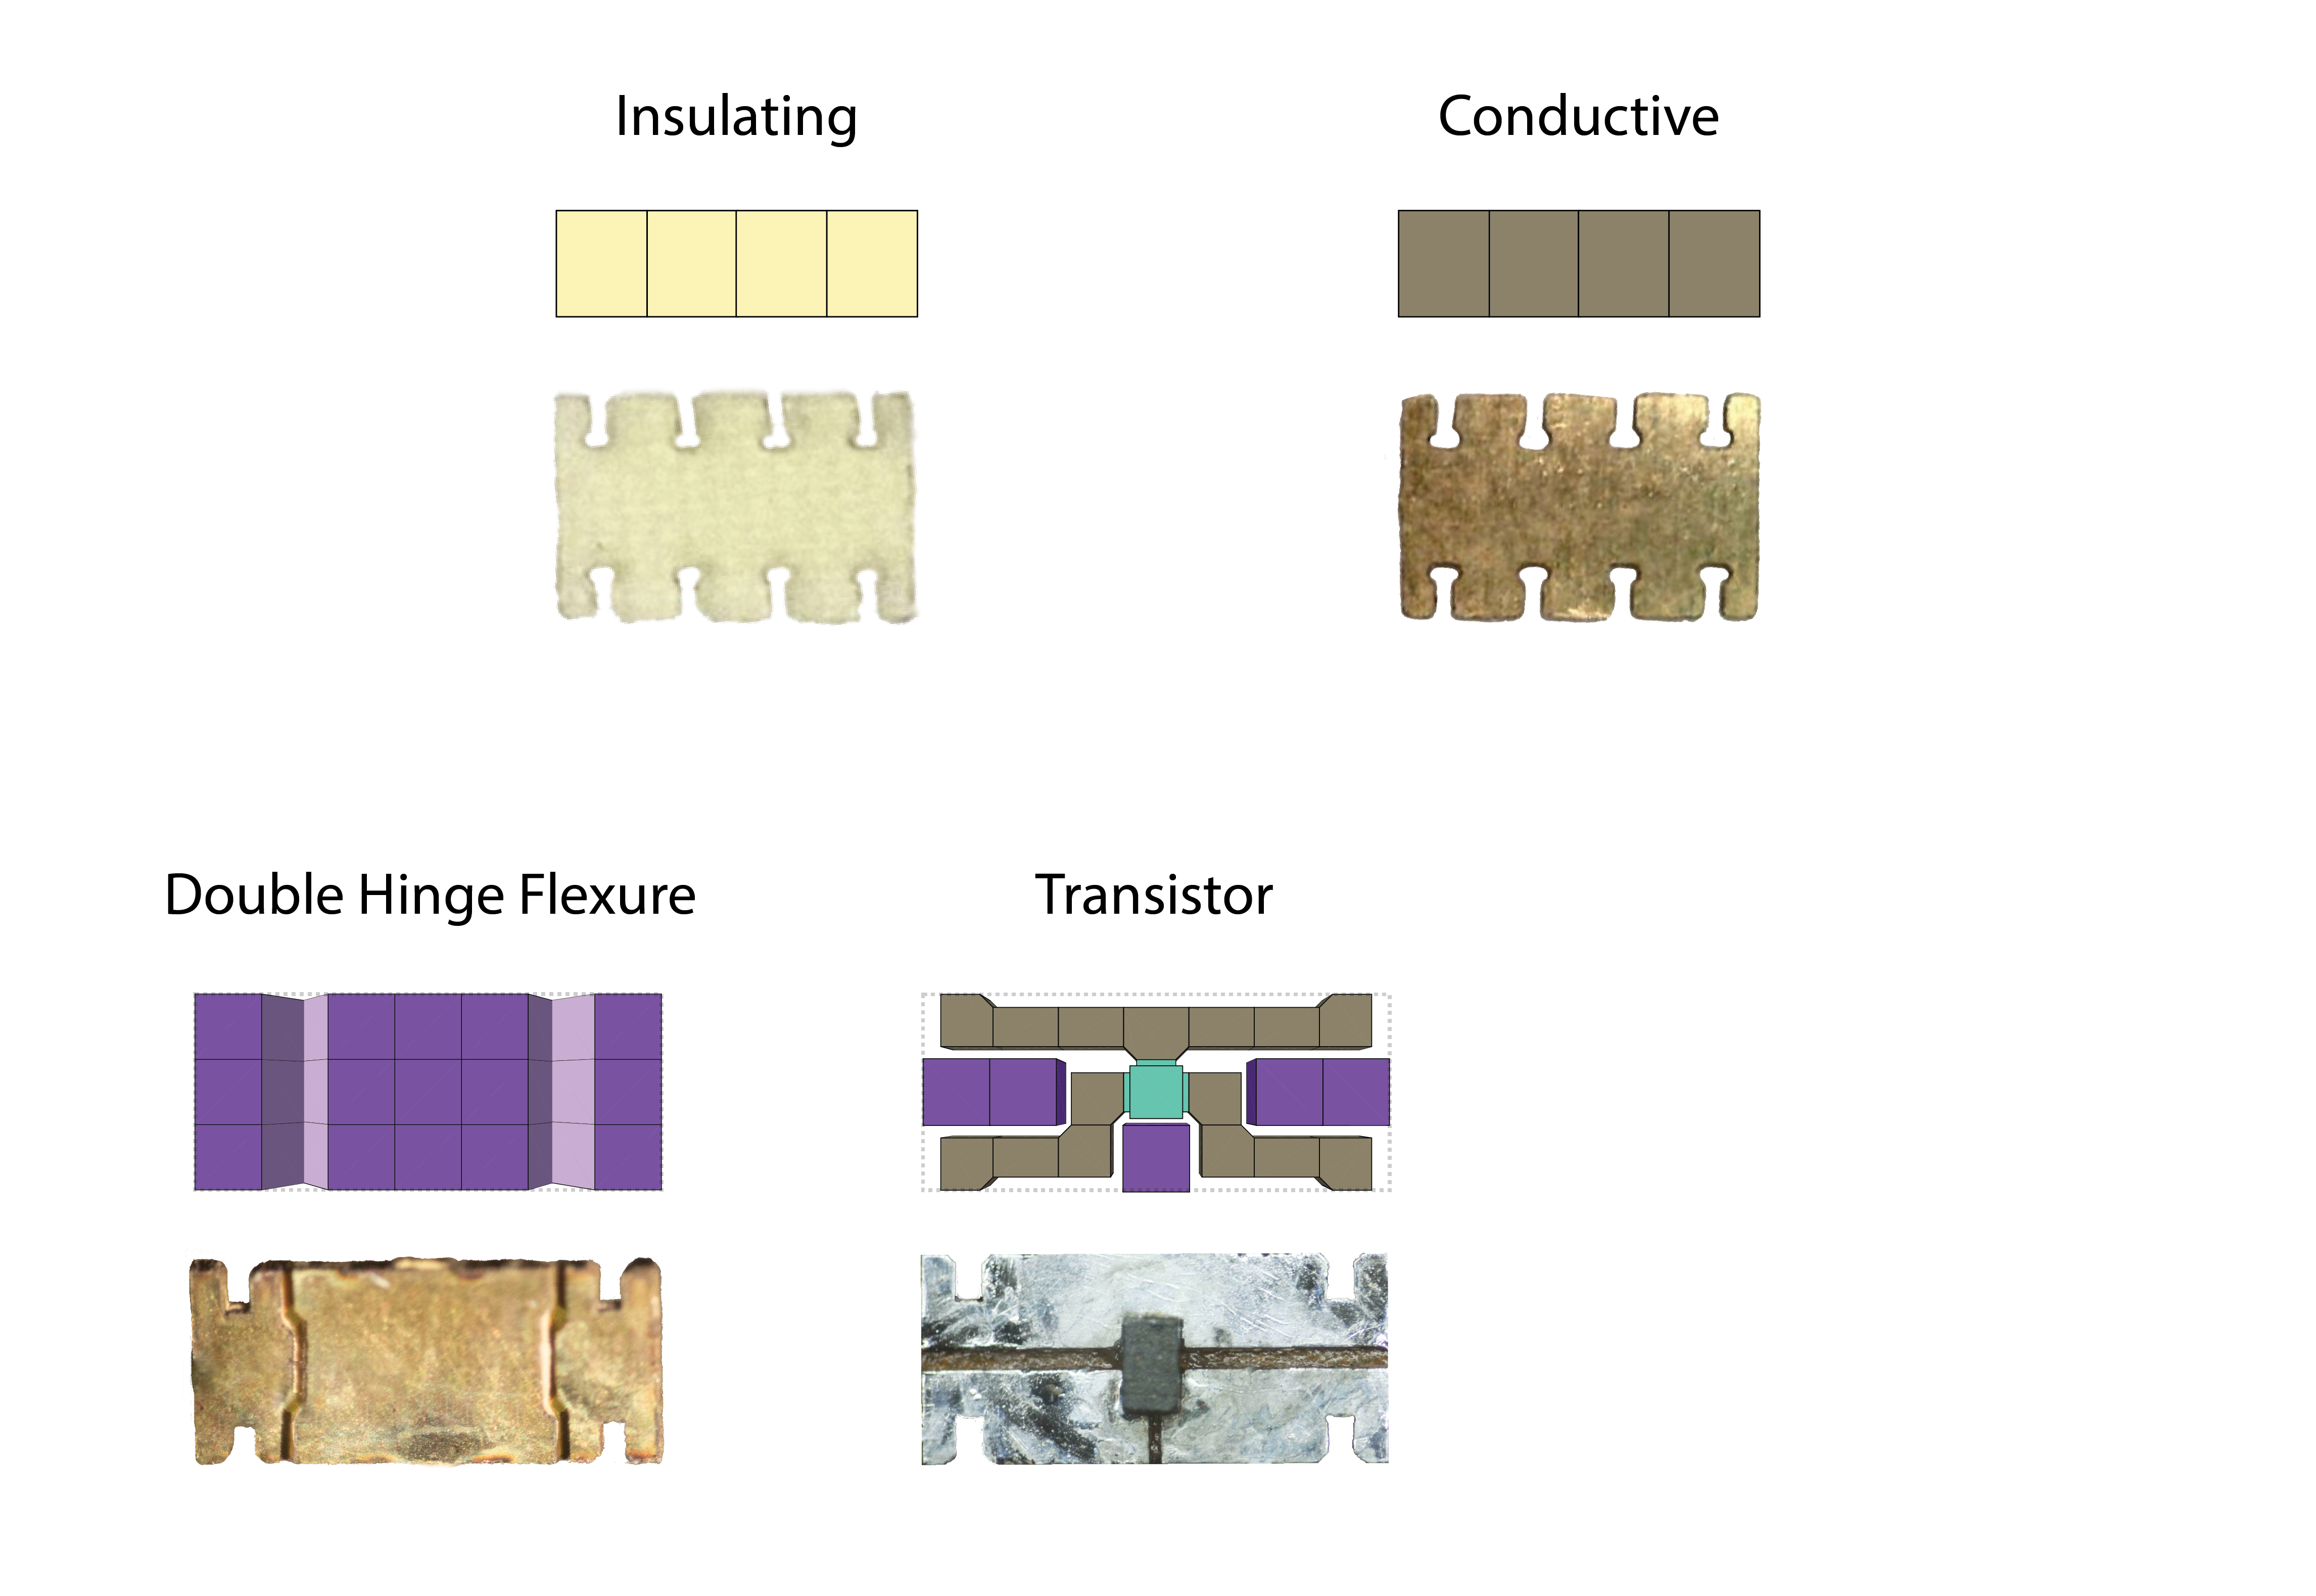
\includegraphics[width=\linewidth]{FunctionalGikIRL.png}
  \caption{FunctionalGikIRL.png.}
  \label{fig:FunctionalGikIRL}
\end{figure}

\section{Hierarchy}

\begin{figure}
  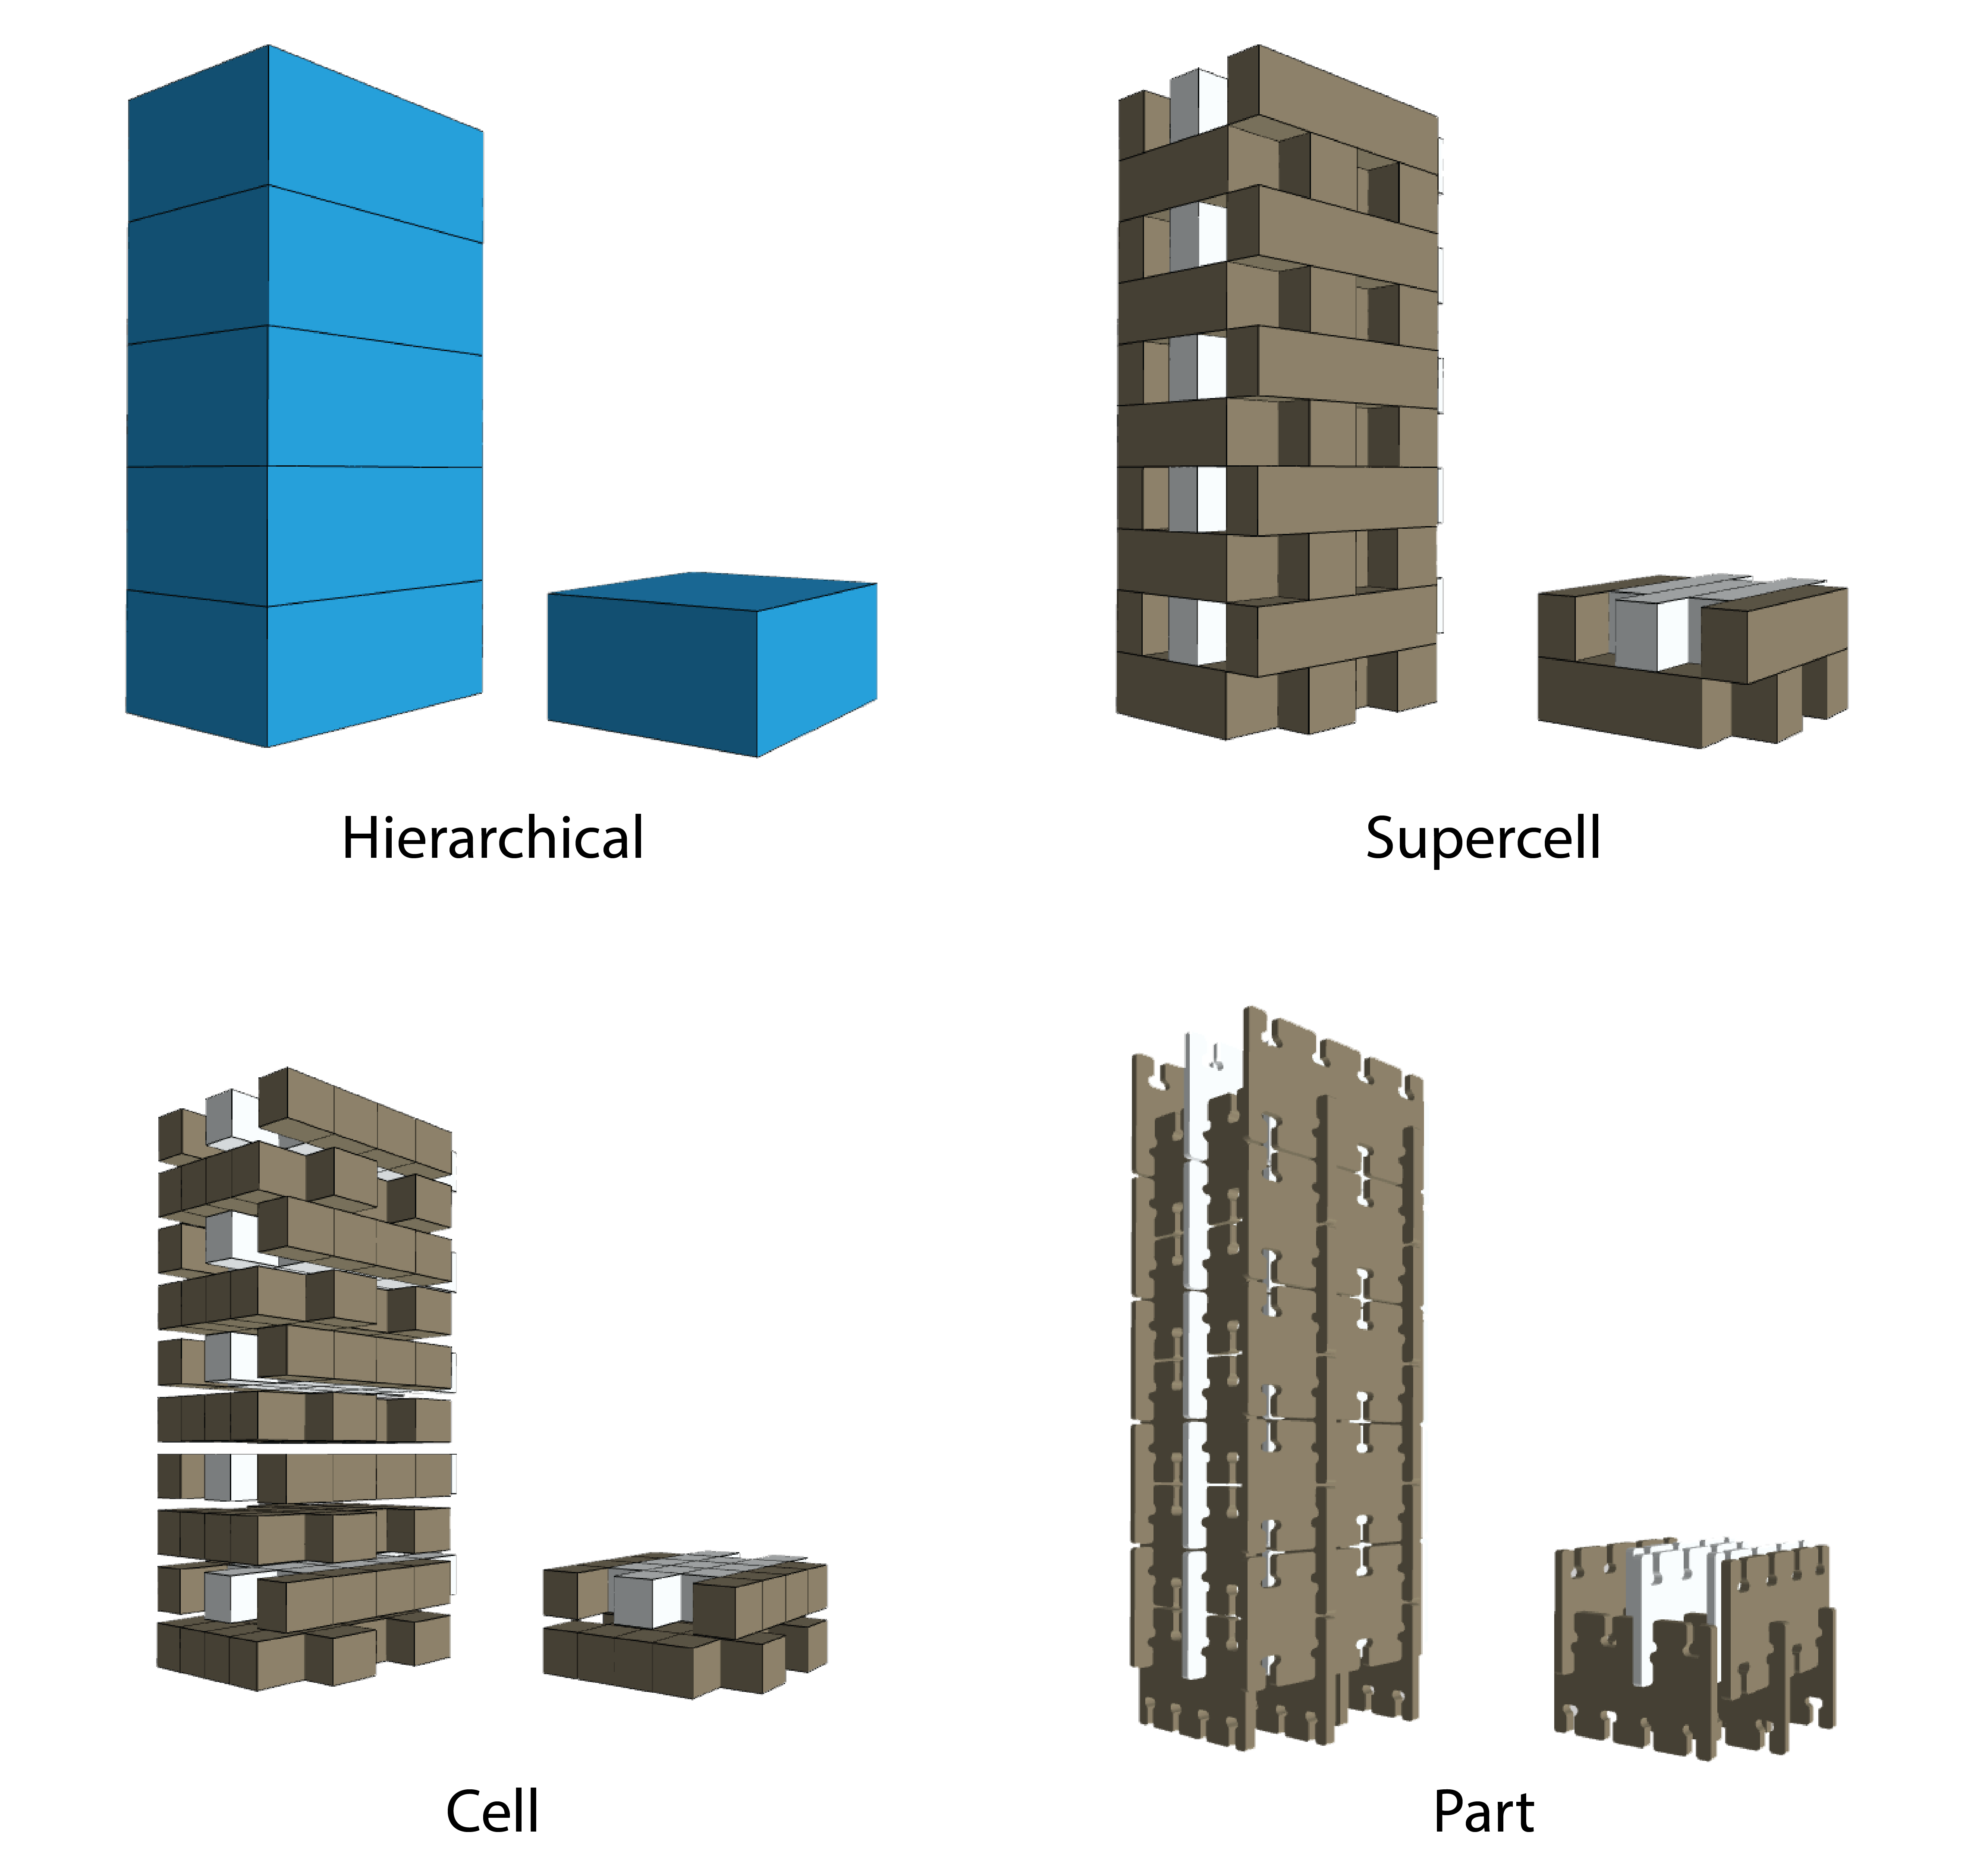
\includegraphics[width=\linewidth]{HierarchyGik.png}
  \caption{HierarchyGik.png.}
  \label{fig:HierarchyGik}
\end{figure}

\section{CAM Workflows}

}
